\documentclass[twoside]{book}

% Packages required by doxygen
\usepackage{fixltx2e}
\usepackage{calc}
\usepackage{doxygen}
\usepackage[export]{adjustbox} % also loads graphicx
\usepackage{graphicx}
\usepackage[utf8]{inputenc}
\usepackage{makeidx}
\usepackage{multicol}
\usepackage{multirow}
\PassOptionsToPackage{warn}{textcomp}
\usepackage{textcomp}
\usepackage[nointegrals]{wasysym}
\usepackage[table]{xcolor}

% Font selection
\usepackage[T1]{fontenc}
\usepackage[scaled=.90]{helvet}
\usepackage{courier}
\usepackage{amssymb}
\usepackage{sectsty}
\renewcommand{\familydefault}{\sfdefault}
\allsectionsfont{%
  \fontseries{bc}\selectfont%
  \color{darkgray}%
}
\renewcommand{\DoxyLabelFont}{%
  \fontseries{bc}\selectfont%
  \color{darkgray}%
}
\newcommand{\+}{\discretionary{\mbox{\scriptsize$\hookleftarrow$}}{}{}}

% Page & text layout
\usepackage{geometry}
\geometry{%
  a4paper,%
  top=2.5cm,%
  bottom=2.5cm,%
  left=2.5cm,%
  right=2.5cm%
}
\tolerance=750
\hfuzz=15pt
\hbadness=750
\setlength{\emergencystretch}{15pt}
\setlength{\parindent}{0cm}
\setlength{\parskip}{3ex plus 2ex minus 2ex}
\makeatletter
\renewcommand{\paragraph}{%
  \@startsection{paragraph}{4}{0ex}{-1.0ex}{1.0ex}{%
    \normalfont\normalsize\bfseries\SS@parafont%
  }%
}
\renewcommand{\subparagraph}{%
  \@startsection{subparagraph}{5}{0ex}{-1.0ex}{1.0ex}{%
    \normalfont\normalsize\bfseries\SS@subparafont%
  }%
}
\makeatother

% Headers & footers
\usepackage{fancyhdr}
\pagestyle{fancyplain}
\fancyhead[LE]{\fancyplain{}{\bfseries\thepage}}
\fancyhead[CE]{\fancyplain{}{}}
\fancyhead[RE]{\fancyplain{}{\bfseries\leftmark}}
\fancyhead[LO]{\fancyplain{}{\bfseries\rightmark}}
\fancyhead[CO]{\fancyplain{}{}}
\fancyhead[RO]{\fancyplain{}{\bfseries\thepage}}
\fancyfoot[LE]{\fancyplain{}{}}
\fancyfoot[CE]{\fancyplain{}{}}
\fancyfoot[RE]{\fancyplain{}{\bfseries\scriptsize Generated by Doxygen }}
\fancyfoot[LO]{\fancyplain{}{\bfseries\scriptsize Generated by Doxygen }}
\fancyfoot[CO]{\fancyplain{}{}}
\fancyfoot[RO]{\fancyplain{}{}}
\renewcommand{\footrulewidth}{0.4pt}
\renewcommand{\chaptermark}[1]{%
  \markboth{#1}{}%
}
\renewcommand{\sectionmark}[1]{%
  \markright{\thesection\ #1}%
}

% Indices & bibliography
\usepackage{natbib}
\usepackage[titles]{tocloft}
\setcounter{tocdepth}{3}
\setcounter{secnumdepth}{5}
\makeindex

% Hyperlinks (required, but should be loaded last)
\usepackage{ifpdf}
\ifpdf
  \usepackage[pdftex,pagebackref=true]{hyperref}
\else
  \usepackage[ps2pdf,pagebackref=true]{hyperref}
\fi
\hypersetup{%
  colorlinks=true,%
  linkcolor=blue,%
  citecolor=blue,%
  unicode%
}

% Custom commands
\newcommand{\clearemptydoublepage}{%
  \newpage{\pagestyle{empty}\cleardoublepage}%
}

\usepackage{caption}
\captionsetup{labelsep=space,justification=centering,font={bf},singlelinecheck=off,skip=4pt,position=top}

%===== C O N T E N T S =====

\begin{document}

% Titlepage & ToC
\hypersetup{pageanchor=false,
             bookmarksnumbered=true,
             pdfencoding=unicode
            }
\pagenumbering{roman}
\begin{titlepage}
\vspace*{7cm}
\begin{center}%
{\Large PhysK }\\
\vspace*{1cm}
{\large Generated by Doxygen 1.8.11}\\
\end{center}
\end{titlepage}
\clearemptydoublepage
\tableofcontents
\clearemptydoublepage
\pagenumbering{arabic}
\hypersetup{pageanchor=true}

%--- Begin generated contents ---
\chapter{Namespace Index}
\section{Packages}
Here are the packages with brief descriptions (if available)\+:\begin{DoxyCompactList}
\item\contentsline{section}{\hyperlink{namespace_phys_k}{PhysK} }{\pageref{namespace_phys_k}}{}
\end{DoxyCompactList}

\chapter{Hierarchical Index}
\section{Class Hierarchy}
This inheritance list is sorted roughly, but not completely, alphabetically\+:\begin{DoxyCompactList}
\item Game\begin{DoxyCompactList}
\item \contentsline{section}{Phys\+K.\+Game\+Application}{\pageref{class_phys_k_1_1_game_application}}{}
\end{DoxyCompactList}
\item \contentsline{section}{Phys\+K.\+Spatial\+Grid}{\pageref{class_phys_k_1_1_spatial_grid}}{}
\item \contentsline{section}{Phys\+K.\+Sprite}{\pageref{class_phys_k_1_1_sprite}}{}
\begin{DoxyCompactList}
\item \contentsline{section}{Phys\+K.\+Physics\+Sprite}{\pageref{class_phys_k_1_1_physics_sprite}}{}
\end{DoxyCompactList}
\item \contentsline{section}{Phys\+K.\+World}{\pageref{class_phys_k_1_1_world}}{}
\end{DoxyCompactList}

\chapter{Class Index}
\section{Class List}
Here are the classes, structs, unions and interfaces with brief descriptions\+:\begin{DoxyCompactList}
\item\contentsline{section}{\hyperlink{class_phys_k_1_1_game_application}{Phys\+K.\+Game\+Application} }{\pageref{class_phys_k_1_1_game_application}}{}
\item\contentsline{section}{\hyperlink{class_phys_k_1_1_physics_sprite}{Phys\+K.\+Physics\+Sprite} }{\pageref{class_phys_k_1_1_physics_sprite}}{}
\item\contentsline{section}{\hyperlink{class_phys_k_1_1_spatial_grid}{Phys\+K.\+Spatial\+Grid} }{\pageref{class_phys_k_1_1_spatial_grid}}{}
\item\contentsline{section}{\hyperlink{class_phys_k_1_1_sprite}{Phys\+K.\+Sprite} }{\pageref{class_phys_k_1_1_sprite}}{}
\item\contentsline{section}{\hyperlink{class_phys_k_1_1_world}{Phys\+K.\+World} }{\pageref{class_phys_k_1_1_world}}{}
\end{DoxyCompactList}

\chapter{Namespace Documentation}
\hypertarget{namespace_phys_k}{}\section{PhysK Namespace Reference}
\label{namespace_phys_k}\index{PhysK@{PhysK}}
\subsection*{Classes}
\begin{DoxyCompactItemize}
\item 
class \hyperlink{class_phys_k_1_1_game_application}{Game\+Application}
\item 
class \hyperlink{class_phys_k_1_1_physics_sprite}{Physics\+Sprite}
\item 
class \hyperlink{class_phys_k_1_1_spatial_grid}{Spatial\+Grid}
\item 
class \hyperlink{class_phys_k_1_1_sprite}{Sprite}
\item 
class \hyperlink{class_phys_k_1_1_world}{World}
\end{DoxyCompactItemize}

\chapter{Class Documentation}
\hypertarget{class_phys_k_1_1_game_application}{}\section{Phys\+K.\+Game\+Application Class Reference}
\label{class_phys_k_1_1_game_application}\index{Phys\+K.\+Game\+Application@{Phys\+K.\+Game\+Application}}
Inheritance diagram for Phys\+K.\+Game\+Application\+:\begin{figure}[H]
\begin{center}
\leavevmode
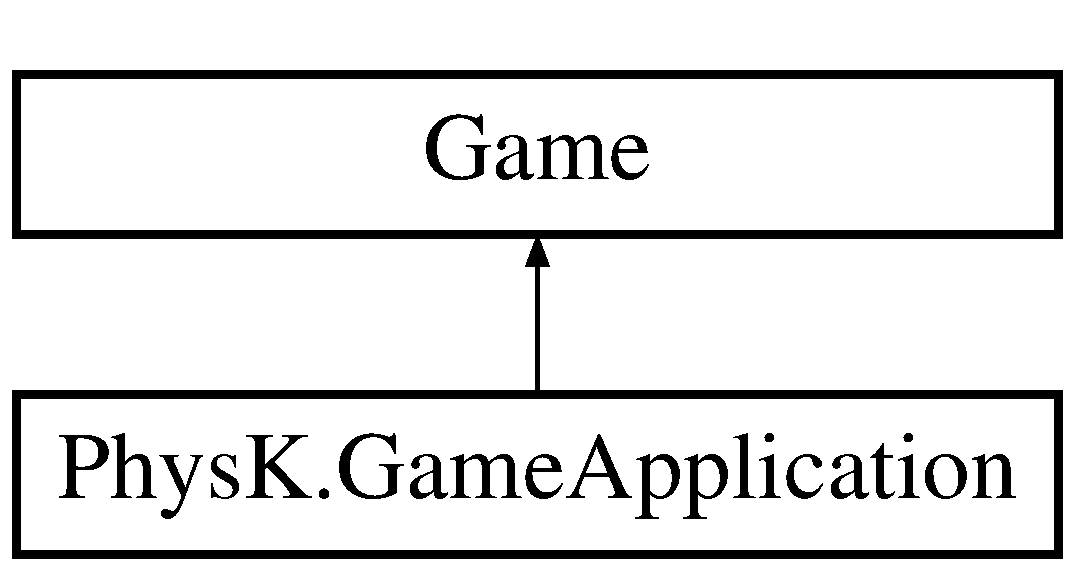
\includegraphics[height=2.000000cm]{class_phys_k_1_1_game_application}
\end{center}
\end{figure}
\subsection*{Static Public Attributes}
\begin{DoxyCompactItemize}
\item 
static Sprite\+Font {\bfseries font}\hypertarget{class_phys_k_1_1_game_application_aaf3a468d312659adf60dda6c9f9db9d7}{}\label{class_phys_k_1_1_game_application_aaf3a468d312659adf60dda6c9f9db9d7}

\end{DoxyCompactItemize}
\subsection*{Protected Member Functions}
\begin{DoxyCompactItemize}
\item 
override void {\bfseries Initialize} ()\hypertarget{class_phys_k_1_1_game_application_a3b3811ce806ca5d00c3ee63ca223db61}{}\label{class_phys_k_1_1_game_application_a3b3811ce806ca5d00c3ee63ca223db61}

\item 
override void {\bfseries Load\+Content} ()\hypertarget{class_phys_k_1_1_game_application_a12d154ea239feafcb1f684b0a2332e20}{}\label{class_phys_k_1_1_game_application_a12d154ea239feafcb1f684b0a2332e20}

\item 
override void {\bfseries Unload\+Content} ()\hypertarget{class_phys_k_1_1_game_application_a5d385e16e5dd5a5b3ab6bf8ce0b8c70f}{}\label{class_phys_k_1_1_game_application_a5d385e16e5dd5a5b3ab6bf8ce0b8c70f}

\item 
override void {\bfseries Update} (Game\+Time game\+Time)\hypertarget{class_phys_k_1_1_game_application_a6fd86dfa9ddbecbb7c6e856ca6384b2f}{}\label{class_phys_k_1_1_game_application_a6fd86dfa9ddbecbb7c6e856ca6384b2f}

\item 
override void {\bfseries Draw} (Game\+Time game\+Time)\hypertarget{class_phys_k_1_1_game_application_a5871c20adb8aa224a4eb0f6e33237c93}{}\label{class_phys_k_1_1_game_application_a5871c20adb8aa224a4eb0f6e33237c93}

\end{DoxyCompactItemize}


The documentation for this class was generated from the following file\+:\begin{DoxyCompactItemize}
\item 
Phys\+K/\+Phys\+K/\+Phys\+K/Game\+Application.\+cs\end{DoxyCompactItemize}

\hypertarget{class_phys_k_1_1_physics_sprite}{}\section{Phys\+K.\+Physics\+Sprite Class Reference}
\label{class_phys_k_1_1_physics_sprite}\index{Phys\+K.\+Physics\+Sprite@{Phys\+K.\+Physics\+Sprite}}
Inheritance diagram for Phys\+K.\+Physics\+Sprite\+:\begin{figure}[H]
\begin{center}
\leavevmode
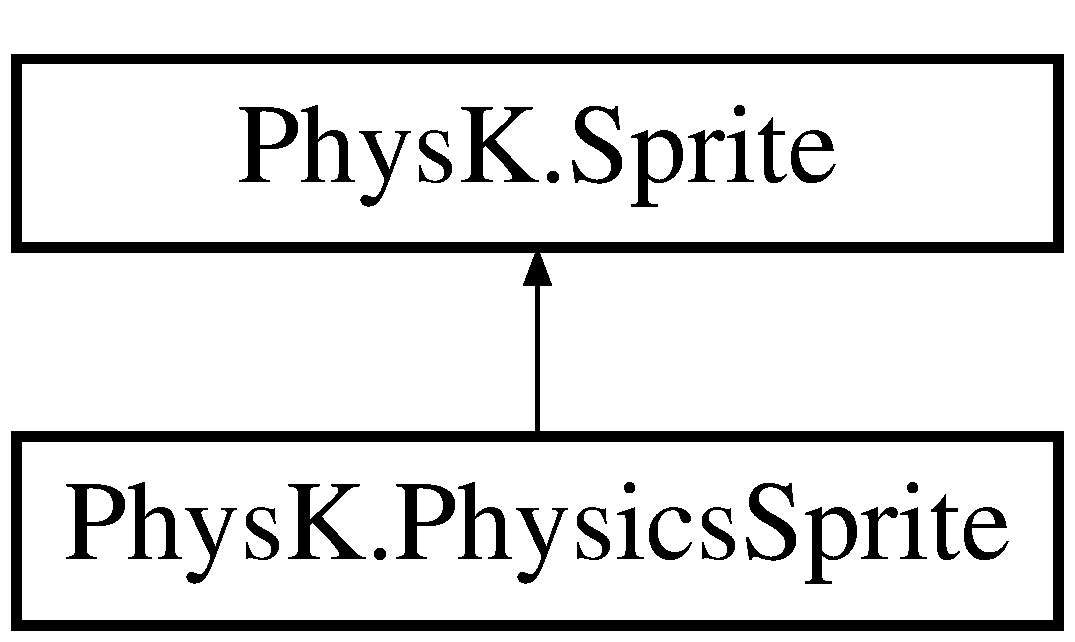
\includegraphics[height=2.000000cm]{class_phys_k_1_1_physics_sprite}
\end{center}
\end{figure}
\subsection*{Public Member Functions}
\begin{DoxyCompactItemize}
\item 
{\bfseries Physics\+Sprite} (Texture2D texture, Vector2 position, Color color, Vector2 velocity, float mass, float restitution)\hypertarget{class_phys_k_1_1_physics_sprite_a44aad16a56a238c79a152d8054da916e}{}\label{class_phys_k_1_1_physics_sprite_a44aad16a56a238c79a152d8054da916e}

\item 
void {\bfseries Debug\+Draw} (Sprite\+Batch sprite\+Batch)\hypertarget{class_phys_k_1_1_physics_sprite_a44514ba961775c5d5f92842936078fd3}{}\label{class_phys_k_1_1_physics_sprite_a44514ba961775c5d5f92842936078fd3}

\item 
void {\bfseries Update} (Game\+Time game\+Time)\hypertarget{class_phys_k_1_1_physics_sprite_a3ddcb5b1e5808270108859f7a374ab0c}{}\label{class_phys_k_1_1_physics_sprite_a3ddcb5b1e5808270108859f7a374ab0c}

\end{DoxyCompactItemize}
\subsection*{Properties}
\begin{DoxyCompactItemize}
\item 
Vector2 {\bfseries Velocity}\hspace{0.3cm}{\ttfamily  \mbox{[}get, set\mbox{]}}\hypertarget{class_phys_k_1_1_physics_sprite_ae744d56fde8d1df7fb0e823312b5a697}{}\label{class_phys_k_1_1_physics_sprite_ae744d56fde8d1df7fb0e823312b5a697}

\item 
Vector2 {\bfseries Acceleration}\hspace{0.3cm}{\ttfamily  \mbox{[}get, set\mbox{]}}\hypertarget{class_phys_k_1_1_physics_sprite_a5e52864eb9c4df5cca3a20765de0152b}{}\label{class_phys_k_1_1_physics_sprite_a5e52864eb9c4df5cca3a20765de0152b}

\item 
float {\bfseries Angular\+Velocity}\hspace{0.3cm}{\ttfamily  \mbox{[}get, set\mbox{]}}\hypertarget{class_phys_k_1_1_physics_sprite_add04efa899bff88b412ed84292bd48e8}{}\label{class_phys_k_1_1_physics_sprite_add04efa899bff88b412ed84292bd48e8}

\item 
float {\bfseries Angular\+Acceleration}\hspace{0.3cm}{\ttfamily  \mbox{[}get, set\mbox{]}}\hypertarget{class_phys_k_1_1_physics_sprite_a95110884f33a8daffb5fbde10712e212}{}\label{class_phys_k_1_1_physics_sprite_a95110884f33a8daffb5fbde10712e212}

\item 
List$<$ Vector2 $>$ {\bfseries Forces}\hspace{0.3cm}{\ttfamily  \mbox{[}get, set\mbox{]}}\hypertarget{class_phys_k_1_1_physics_sprite_aed4d14fb8f0d71c8a717d4369ce6ce7c}{}\label{class_phys_k_1_1_physics_sprite_aed4d14fb8f0d71c8a717d4369ce6ce7c}

\item 
float {\bfseries Mass}\hspace{0.3cm}{\ttfamily  \mbox{[}get, set\mbox{]}}\hypertarget{class_phys_k_1_1_physics_sprite_aee78d23703a1fff5651d28a2a29b8889}{}\label{class_phys_k_1_1_physics_sprite_aee78d23703a1fff5651d28a2a29b8889}

\item 
float {\bfseries Restitution}\hspace{0.3cm}{\ttfamily  \mbox{[}get, set\mbox{]}}\hypertarget{class_phys_k_1_1_physics_sprite_aa99fd17f5a8705da6090de795cc489b7}{}\label{class_phys_k_1_1_physics_sprite_aa99fd17f5a8705da6090de795cc489b7}

\item 
Rectangle {\bfseries Alligned\+Hitbox}\hspace{0.3cm}{\ttfamily  \mbox{[}get, set\mbox{]}}\hypertarget{class_phys_k_1_1_physics_sprite_a74026774de649a349d0c5fcdaececcf6}{}\label{class_phys_k_1_1_physics_sprite_a74026774de649a349d0c5fcdaececcf6}

\item 
Vector2 {\bfseries Center}\hspace{0.3cm}{\ttfamily  \mbox{[}get, set\mbox{]}}\hypertarget{class_phys_k_1_1_physics_sprite_adb710fdf51c89dd500940d04c2c4a41f}{}\label{class_phys_k_1_1_physics_sprite_adb710fdf51c89dd500940d04c2c4a41f}

\item 
float {\bfseries Radius}\hspace{0.3cm}{\ttfamily  \mbox{[}get, set\mbox{]}}\hypertarget{class_phys_k_1_1_physics_sprite_a67d012f8d8364de0c9b50da9c1b80771}{}\label{class_phys_k_1_1_physics_sprite_a67d012f8d8364de0c9b50da9c1b80771}

\item 
Vector2 {\bfseries Momentum}\hspace{0.3cm}{\ttfamily  \mbox{[}get\mbox{]}}\hypertarget{class_phys_k_1_1_physics_sprite_a43db585d8210c156cc6123c93ce663f6}{}\label{class_phys_k_1_1_physics_sprite_a43db585d8210c156cc6123c93ce663f6}

\end{DoxyCompactItemize}
\subsection*{Additional Inherited Members}


The documentation for this class was generated from the following file\+:\begin{DoxyCompactItemize}
\item 
Phys\+K/\+Phys\+K/\+Phys\+K/Physics\+Sprite.\+cs\end{DoxyCompactItemize}

\hypertarget{class_phys_k_1_1_spatial_grid}{}\section{Phys\+K.\+Spatial\+Grid Class Reference}
\label{class_phys_k_1_1_spatial_grid}\index{Phys\+K.\+Spatial\+Grid@{Phys\+K.\+Spatial\+Grid}}
\subsection*{Properties}
\begin{DoxyCompactItemize}
\item 
Rectangle {\bfseries Bounds}\hspace{0.3cm}{\ttfamily  \mbox{[}get, set\mbox{]}}\hypertarget{class_phys_k_1_1_spatial_grid_a5eee478422a07c9387716400b0516038}{}\label{class_phys_k_1_1_spatial_grid_a5eee478422a07c9387716400b0516038}

\item 
List$<$ \hyperlink{class_phys_k_1_1_physics_sprite}{Physics\+Sprite} $>$ {\bfseries Items}\hspace{0.3cm}{\ttfamily  \mbox{[}get, set\mbox{]}}\hypertarget{class_phys_k_1_1_spatial_grid_a11c95e5b2bbf2556e3306106627bde92}{}\label{class_phys_k_1_1_spatial_grid_a11c95e5b2bbf2556e3306106627bde92}

\end{DoxyCompactItemize}


The documentation for this class was generated from the following file\+:\begin{DoxyCompactItemize}
\item 
Phys\+K/\+Phys\+K/\+Phys\+K/Spatial\+Grid.\+cs\end{DoxyCompactItemize}

\hypertarget{class_phys_k_1_1_sprite}{}\section{Phys\+K.\+Sprite Class Reference}
\label{class_phys_k_1_1_sprite}\index{Phys\+K.\+Sprite@{Phys\+K.\+Sprite}}
Inheritance diagram for Phys\+K.\+Sprite\+:\begin{figure}[H]
\begin{center}
\leavevmode
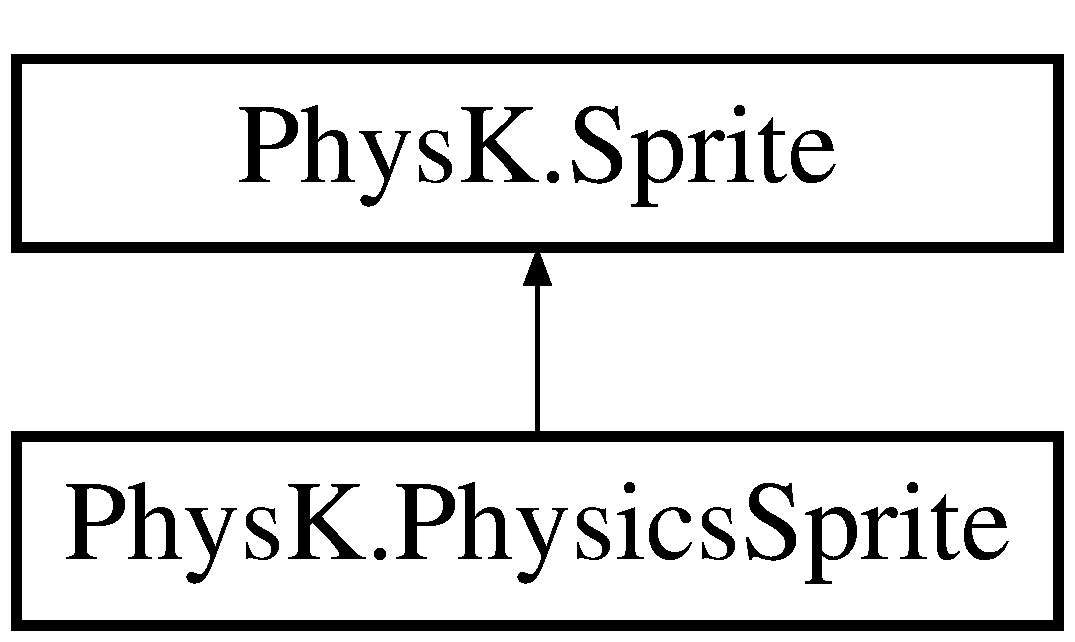
\includegraphics[height=2.000000cm]{class_phys_k_1_1_sprite}
\end{center}
\end{figure}
\subsection*{Public Member Functions}
\begin{DoxyCompactItemize}
\item 
{\bfseries Sprite} (Texture2D texture, Vector2 position, Rectangle source\+Rectangle, Color color, float rotation, Vector2 origin, Vector2 scale, float layer\+Depth)\hypertarget{class_phys_k_1_1_sprite_a06eb35aaa1194dd46b7aaf580f1cd867}{}\label{class_phys_k_1_1_sprite_a06eb35aaa1194dd46b7aaf580f1cd867}

\item 
{\bfseries Sprite} (Texture2D texture, Vector2 position, Color color)\hypertarget{class_phys_k_1_1_sprite_acd414c011a44f85b6dc03a4c0f876ba0}{}\label{class_phys_k_1_1_sprite_acd414c011a44f85b6dc03a4c0f876ba0}

\item 
virtual void {\bfseries Draw} (Sprite\+Batch sprite\+Batch)\hypertarget{class_phys_k_1_1_sprite_aef86d663292d353f0b76b6623102e07b}{}\label{class_phys_k_1_1_sprite_aef86d663292d353f0b76b6623102e07b}

\end{DoxyCompactItemize}
\subsection*{Protected Attributes}
\begin{DoxyCompactItemize}
\item 
Texture2D {\bfseries texture}\hypertarget{class_phys_k_1_1_sprite_a700ed22d527abcd398cfed27ee0eab3e}{}\label{class_phys_k_1_1_sprite_a700ed22d527abcd398cfed27ee0eab3e}

\item 
Vector2 {\bfseries position}\hypertarget{class_phys_k_1_1_sprite_abc08b4b85e5c7adb45610d6b7d9c5596}{}\label{class_phys_k_1_1_sprite_abc08b4b85e5c7adb45610d6b7d9c5596}

\item 
Rectangle {\bfseries source\+Rectangle}\hypertarget{class_phys_k_1_1_sprite_a0e20a182532b3f51de81d677f8ad9ee7}{}\label{class_phys_k_1_1_sprite_a0e20a182532b3f51de81d677f8ad9ee7}

\item 
Color {\bfseries color}\hypertarget{class_phys_k_1_1_sprite_abe122a062077d1bb8face31da2bb43c4}{}\label{class_phys_k_1_1_sprite_abe122a062077d1bb8face31da2bb43c4}

\item 
float {\bfseries rotation}\hypertarget{class_phys_k_1_1_sprite_a53ede37cf42dc8a8fae8d465c83f508f}{}\label{class_phys_k_1_1_sprite_a53ede37cf42dc8a8fae8d465c83f508f}

\item 
Vector2 {\bfseries origin}\hypertarget{class_phys_k_1_1_sprite_a8901ac895ab2c84e24185d7ec834ed99}{}\label{class_phys_k_1_1_sprite_a8901ac895ab2c84e24185d7ec834ed99}

\item 
Vector2 {\bfseries scale}\hypertarget{class_phys_k_1_1_sprite_ab8683f97d567104eb7b9a696890be4f1}{}\label{class_phys_k_1_1_sprite_ab8683f97d567104eb7b9a696890be4f1}

\item 
Sprite\+Effects {\bfseries effects}\hypertarget{class_phys_k_1_1_sprite_ac8056ded4665d81a5628e90b09ad5c57}{}\label{class_phys_k_1_1_sprite_ac8056ded4665d81a5628e90b09ad5c57}

\item 
float {\bfseries layer\+Depth}\hypertarget{class_phys_k_1_1_sprite_a19dbf7f46015e598e1eb7ef37c4941bb}{}\label{class_phys_k_1_1_sprite_a19dbf7f46015e598e1eb7ef37c4941bb}

\end{DoxyCompactItemize}
\subsection*{Properties}
\begin{DoxyCompactItemize}
\item 
Texture2D {\bfseries Texture}\hspace{0.3cm}{\ttfamily  \mbox{[}get, set\mbox{]}}\hypertarget{class_phys_k_1_1_sprite_afceb0b7330baa642eb875505b7644a9f}{}\label{class_phys_k_1_1_sprite_afceb0b7330baa642eb875505b7644a9f}

\item 
Vector2 {\bfseries Position}\hspace{0.3cm}{\ttfamily  \mbox{[}get, set\mbox{]}}\hypertarget{class_phys_k_1_1_sprite_a3f54c876e5a0983351e26b95c758fd9d}{}\label{class_phys_k_1_1_sprite_a3f54c876e5a0983351e26b95c758fd9d}

\item 
Rectangle {\bfseries Source\+Rectangle}\hspace{0.3cm}{\ttfamily  \mbox{[}get, set\mbox{]}}\hypertarget{class_phys_k_1_1_sprite_af52a20a1c06e924a33b2de25c52d8c4b}{}\label{class_phys_k_1_1_sprite_af52a20a1c06e924a33b2de25c52d8c4b}

\item 
Color {\bfseries Color}\hspace{0.3cm}{\ttfamily  \mbox{[}get, set\mbox{]}}\hypertarget{class_phys_k_1_1_sprite_af4c938e87bc79ed83f226bd6e75290be}{}\label{class_phys_k_1_1_sprite_af4c938e87bc79ed83f226bd6e75290be}

\item 
float {\bfseries Rotation}\hspace{0.3cm}{\ttfamily  \mbox{[}get, set\mbox{]}}\hypertarget{class_phys_k_1_1_sprite_a118a92c52726117a4574ee493bd2cfb9}{}\label{class_phys_k_1_1_sprite_a118a92c52726117a4574ee493bd2cfb9}

\item 
Vector2 {\bfseries Origin}\hspace{0.3cm}{\ttfamily  \mbox{[}get, set\mbox{]}}\hypertarget{class_phys_k_1_1_sprite_a6f3706be4c8d700e27fe4a9eeed6a800}{}\label{class_phys_k_1_1_sprite_a6f3706be4c8d700e27fe4a9eeed6a800}

\item 
Vector2 {\bfseries Scale}\hspace{0.3cm}{\ttfamily  \mbox{[}get, set\mbox{]}}\hypertarget{class_phys_k_1_1_sprite_a98e8ecce2777763a381a395ab256eefe}{}\label{class_phys_k_1_1_sprite_a98e8ecce2777763a381a395ab256eefe}

\item 
Sprite\+Effects {\bfseries Effects}\hspace{0.3cm}{\ttfamily  \mbox{[}get, set\mbox{]}}\hypertarget{class_phys_k_1_1_sprite_a72469c980c72cffb92585489d2fb9be7}{}\label{class_phys_k_1_1_sprite_a72469c980c72cffb92585489d2fb9be7}

\item 
float {\bfseries Layer\+Depth}\hspace{0.3cm}{\ttfamily  \mbox{[}get, set\mbox{]}}\hypertarget{class_phys_k_1_1_sprite_a76feb08a54791bcfa90b0a472a15e892}{}\label{class_phys_k_1_1_sprite_a76feb08a54791bcfa90b0a472a15e892}

\end{DoxyCompactItemize}


The documentation for this class was generated from the following file\+:\begin{DoxyCompactItemize}
\item 
Phys\+K/\+Phys\+K/\+Phys\+K/Sprite.\+cs\end{DoxyCompactItemize}

\hypertarget{class_phys_k_1_1_world}{}\section{Phys\+K.\+World Class Reference}
\label{class_phys_k_1_1_world}\index{Phys\+K.\+World@{Phys\+K.\+World}}
\subsection*{Public Member Functions}
\begin{DoxyCompactItemize}
\item 
{\bfseries World} (Graphics\+Device graphics\+Device)\hypertarget{class_phys_k_1_1_world_a32c4a8c2c6f055987352729f5d3d8945}{}\label{class_phys_k_1_1_world_a32c4a8c2c6f055987352729f5d3d8945}

\item 
void {\bfseries Update} (Game\+Time game\+Time)\hypertarget{class_phys_k_1_1_world_a92cae5266d900ee840afbd8fd421e1ca}{}\label{class_phys_k_1_1_world_a92cae5266d900ee840afbd8fd421e1ca}

\item 
void {\bfseries Draw} (Sprite\+Batch sprite\+Batch)\hypertarget{class_phys_k_1_1_world_a62ca116b56748ed477b5c37ffcf5d37b}{}\label{class_phys_k_1_1_world_a62ca116b56748ed477b5c37ffcf5d37b}

\end{DoxyCompactItemize}
\subsection*{Static Public Attributes}
\begin{DoxyCompactItemize}
\item 
static Texture2D {\bfseries pixel}\hypertarget{class_phys_k_1_1_world_a5ac853e0538bde0bad91879721fbbf54}{}\label{class_phys_k_1_1_world_a5ac853e0538bde0bad91879721fbbf54}

\end{DoxyCompactItemize}
\subsection*{Properties}
\begin{DoxyCompactItemize}
\item 
\hyperlink{class_phys_k_1_1_physics_sprite}{Physics\+Sprite}\mbox{[}$\,$\mbox{]} {\bfseries Items}\hspace{0.3cm}{\ttfamily  \mbox{[}get, set\mbox{]}}\hypertarget{class_phys_k_1_1_world_a04e7b4abd4acc5081b12628509a68eff}{}\label{class_phys_k_1_1_world_a04e7b4abd4acc5081b12628509a68eff}

\item 
Rectangle {\bfseries Bounds}\hspace{0.3cm}{\ttfamily  \mbox{[}get, set\mbox{]}}\hypertarget{class_phys_k_1_1_world_ac6f8018610492ff8b2e949bfd9204a95}{}\label{class_phys_k_1_1_world_ac6f8018610492ff8b2e949bfd9204a95}

\end{DoxyCompactItemize}


The documentation for this class was generated from the following file\+:\begin{DoxyCompactItemize}
\item 
Phys\+K/\+Phys\+K/\+Phys\+K/World.\+cs\end{DoxyCompactItemize}

%--- End generated contents ---

% Index
\backmatter
\newpage
\phantomsection
\clearemptydoublepage
\addcontentsline{toc}{chapter}{Index}
\printindex

\end{document}
